    機械学習とは,特定課題に対してコンピュータが効率よく動作するようなパターンを見つけるアルゴリズムまたは統計モデルの研究分野であり,人工知能研究の一つとして数えられる.
    機械学習はルールベースのアルゴリズムなどとは異なり,アルゴリズムが人間に判断基準を明示されることなく,判断基準をデータから見つけるような動作をするアルゴリズムのことである.
    機械学習の父とも呼ばれるアーサー・サミュエルによれば,機械学習は
    \begin{quote}
        Field of study that gives computers the ability to learn without being explicitly programmed
        
        明示的にプログラムしなくても学習する能力をコンピュータに与える研究分野
    \end{quote}
    であると定義されている\cite{samuel1959some}.さらに,具体的には経験$(E)$に基づいて,精度$(P)$がタスク$(T)$に対して最適化されていくようなアルゴリズムのことを指すとしている.
    
    機械学習は,例えばN個の訓練集合(training set)${\bm{x}_1, \bm{x}_2, \bm{x}_3, ... , \bm{x}_N}$が与えられたとき,それに対応する目標ベクトル(target vector)${\bm{t}_1, \bm{t}_2, \bm{t}_3, ... , \bm{t}_N}$と,訓練集合を用いて予測したベクトル${\bm{y}_1, \bm{y}_2, \bm{y}_3, ... , \bm{y}_N}$の誤差が最小になるような関数$f_w(x)$を得るような操作である.
    このとき,誤差の計算で用いる関数を誤差関数(Error function),コスト関数(Cost function)または損失関数(Loss function)と呼ぶ.
    一度訓練集合と目標ベクトルで訓練されたモデルは,異なるデータ集合に対しても適用可能である.
    例えば,数字認識のモデルでは数字が描かれている画像(訓練集合)と画像に対応する数字(目標ベクトル)が与えられ,分類モデル$y(x)$が得られた場合,訓練集合に無い画像に対してもモデルは数字の予測を行うことが可能である.
    このような訓練集合と異なる新たな事例に対して予測を行う能力のことを汎化(generalization)と呼ぶ.
    以上のような枠組みは教師あり学習と呼ばれ,機械学習の中でも最も良く用いられる手法の一つである.
    
    機械学習は大きく分けて教師あり学習,教師なし学習,強化学習の3つに大別することができる.
    教師あり学習は先程のように訓練集合と目標ベクトルが与えられ,誤算関数を最小化,または汎化するようなモデルを得るような操作のことである.
    これと比べ,教師なし学習はその名の通り目標ベクトルを持たない.
    教師なし学習では,訓練集合の中で似通ったデータをまとめるクラスタリングや,データの次元圧縮などが行われ,それに伴ってデータの視覚化(Visualization)などに活用されることが多い.
    最後の強化学習は,試行錯誤を通じて「価値を最大化するような行動」を学習する手法である.
    これは教師あり学習と同じ目的のように思われるが,教師あり学習とは目標ベクトルが詳細に定義されていない点で異なる.
    強化学習の場合には最終的な目標(例えばゲームに勝利する,電力効率を上げるなど)のみが与えられるタスクや,あらかじめ詳細な目標が分からない(または,取得が困難である)ようなタスクに対してより良い振る舞いをさせることが目標となる.
    
    機械学習の様々な種類について触れたが,単純に機械学習と呼ばれる場合には教師あり学習のことを指す場合が多い.
    教師あり学習には大きく分けて分類と回帰という2つのタスクが存在している.
    教師あり学習におけるこの2つのタスクタイプの顕著な違いは,その出力形式である.
    分類タスクでは出力値は離散値をとり,不連続である.
    これは例えば明日の天気を予測したり,画像から花の種類を予測したりといったタスクが該当する.
    一方,回帰タスクは連続値をとる.
    これには,例えば明日の気温の予測や,数々の条件から家の値段を推測するようなタスクが該当する.
    
    また,この2つのタスクが複合することもありうる.
    近年深層学習の貢献によって大きな発展を遂げた物体検出が顕著な例である.
    物体検出では物体の位置がどこであるかを回帰し,物体な何であるかを分類する.
    また,分類時の確率を出力することは回帰であると捉えることも可能である.
    
    本節では,実際に教師あり学習の枠組みの中の機械学習のアルゴリズムを複数示し,次節に示す深層学習の理解の助けとする.

\subsection{線形回帰}
    線形回帰は最も一般的な機械学習のアルゴリズムであり,このアルゴリズムは名前の通り回帰タスクを実行する.
    このアルゴリズムは訓練集合および目標ベクトルの組み合わせ${\bm{x},\bm{y}}$が与えられたとき,その誤差を最小化するようなパラメータ$\bm{w}$を持つ関数$f_w(\cdot )$を求めるアルゴリズムである.
    
    以下では,簡単のため訓練集合および目標ベクトルをそれぞれ1次元データとして考え,$w_0$(バイアス項)を無視する.
    すると,最適化対象の式(hypothesis)$h(x)$はと以下のように表すことができる.
    \begin{equation}
        h_w(x) = w_0 + w_1 x
    \end{equation}
    よって,あるデータ$(x, y)$についての誤差は以下のように表すことができる.
    \begin{equation}
        Error(w_1) = h_w\left(x\right)-y
    \end{equation}
    訓練集合${x^{(1)}, x^{(2)}, x^{(3)}, ... , x^{(N)}}$および対応する目標値${y^{(1)}, y^{(2)}, y^{(3)}, ... , y^{(4)}}$が与えられ,それぞれに対する誤差の合計値を最小化することを考える.
    つまり,線形回帰における損失関数は以下のようになる.
    \begin{equation}
        L(w_1) = \frac{1}{2N}\sum_{i=1}^{N}\left(h_w (x^{(i)})-y^{(i)}\right)^2
    \end{equation}
    ここで,総和および$1/N$で各誤差の平均をとっていることがわかる.($1/2$が乗算されていることについては後述する.)
    また,単純な誤差の平均ではなく,誤差の二乗を取っていることに注意する.
    これは誤差における符号の影響をなくすために用いられる.
    平均二乗誤差(Mean Square Error)は回帰においてしばしば用いられる損失関数の一つで,二乗ではなく誤差の絶対値を用いる手法を平均絶対値誤差(Mean Absolute Error)と呼ぶ.
    
    \begin{figure}[t]
        \begin{center}
            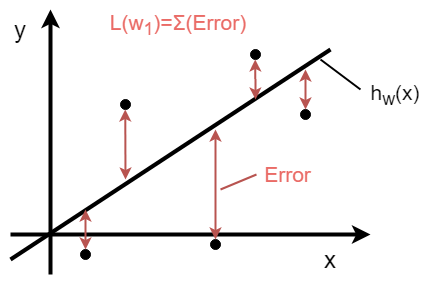
\includegraphics[width=8.0cm]{./8_appendix/img/error}
            \caption{Simplified diagram of the loss function in linear regression.}
            \label{2_linerregression_loss}
        \end{center}
    \end{figure}
    
    さて,次にこの損失関数を最小化する方法を考える.
    $h_w(x)=w_1 x$より,先程の損失関数は以下のように表すことができる.
    \begin{equation}
        L(w_1) = \frac{1}{2N}\sum_{i=1}^{N}\left(w_1 x^{(i)} - y^{(i)}\right)^2
    \end{equation}
    上記の式において,$x^{(i)}$ および $y^{(i)}$は既知の値であることから,$L(w_1)$は$w_1$に関する下に凸の2次関数となることが分かる.
    つまり,線形回帰において最小二乗誤差を最小化することは,損失関数の微分値が0になる値を求めることと等価である.
    
    さて,先程は2つの大きな仮定を用いて数式を単純化した.
    一つは訓練集合が1次元であるという仮定.
    もう一つは$w_0$(バイアス項)が0であるという仮定である.
    実際には訓練集合は多変数である場合がほとんどであり,バイアス項を考慮しないと精度の良いモデルは得られない.
    以降では多変数の場合の線形回帰について見ていく.
    
    多変数を考える線形回帰は特に重回帰分析と呼ばれ,最適化対象の式(hypothesis)$h(x)$は,以下のように表すことができる.
    \begin{equation}
        h_{\bm{w}}(\bm{x}) = w_0・1 + w_1 x_1 + w_2 x_2 + ...  + w_d x_d = \bm{w}^T\bm{x}
    \end{equation}
    このような多項式は線形モデルとも呼ばれる.
    線形モデルに関して,損失関数は同様に以下のように定義される.
    ここで$\bm{x}=(x_1, x_2, x_3, ... , x_d)$であることに注意する.
    \begin{equation}
        L(\bm{w}) = \frac{1}{2N}\sum_{i=1}^{N}\left(h_{\bm{w}}(\bm{x}^{(i)})-y^{(i)}\right)^2
        \label{linerregression_loss_equation}
    \end{equation}
    先程,線形回帰においては最小二乗誤差を最小化することは,損失関数の微分値が0になる値を求めることと等価であると述べた.
    これは重回帰分析においても同様であり,パラメータ$\bm{w}$は以下の式を解くことによって導出できる.
    \begin{equation}
        \frac{\partial L(\boldsymbol{w})}{\partial \boldsymbol{w}}=\frac{\partial}{\partial \boldsymbol{w}} \frac{1}{2N} \sum_{i=1}^{N}\left(h_{\boldsymbol{w}}(\boldsymbol{x}^{(\boldsymbol{i})})-y_{n}\right)^{2}=\mathbf{0}
    \end{equation}
    ここで,訓練集合について,以下で定義される行列のことを慣習として計画行列(デザイン行列)と呼び,$\Phi$で表す.
    
    \begin{equation}
        \bm{\Phi}=\left(
            \begin{array}{ccccc}
                1 & x^{(1)}_1 & x^{(1)}_2 & \cdots & x^{(1)}_d \\
                1 & x^{(2)}_1 & x^{(2)}_2 & \cdots & x^{(2)}_d \\
                1 & x^{(3)}_1 & x^{(3)}_2 & \cdots & x^{(3)}_d \\
                \vdots & \vdots & \vdots & \ddots & \vdots \\
                1 & x^{(N)}_1 & x^{(N)}_2 & \cdots & x^{(N)}_d
            \end{array}\right)
    \end{equation}
    
    これを用いて先程の損失関数を表すと,以下のようになる.
    \begin{eqnarray}
        L(\bm{w}) &=& \frac{1}{2N}\left( \bm{w\Phi} - \bm{y} \right)^2\  =\  \frac{1}{2N}\left( \bm{w\Phi} - \bm{y} \right)^T \left( \bm{w\Phi} - \bm{y} \right)\\
        &=& \frac{1}{2N}\left( \bm{w}^T\bm{\Phi}^T - \bm{y}^T \right) \left( \bm{w\Phi} - \bm{y} \right)\\
        &=& \frac{1}{2}\left(\bm{w}^T \bm{\Phi} \boldsymbol{w}-\boldsymbol{w}^T \bm{\Phi}^T \boldsymbol{y}-\boldsymbol{y}^T \bm{\Phi} \boldsymbol{w}+\boldsymbol{y}^T \boldsymbol{y}\right)\\
        &=& \frac{1}{2}\left(\bm{w}^T \bm{\Phi} \boldsymbol{w}-2\boldsymbol{w}^T \bm{\Phi}^T \boldsymbol{y}+\boldsymbol{y}^T \boldsymbol{y}\right)
    \end{eqnarray}
    つまり,損失関数の微分は以下のように求まる.
    ここで,先程乗算した$1/2$が微分値を簡素な値にしていることに注意する.
    \begin{eqnarray}
        \frac{\partial L(\boldsymbol{w})}{\partial \boldsymbol{w}} 
        &=&\frac{\partial}{\partial \boldsymbol{w}} \frac{1}{2}\left(\boldsymbol{w}^T \bm{\Phi}^T \bm{\Phi} \boldsymbol{w}-2 \boldsymbol{w}^T \bm{\Phi}^T \boldsymbol{y}+\boldsymbol{y}^T \boldsymbol{y}\right) \\
        &=&\frac{1}{2} \frac{\partial}{\partial \boldsymbol{w}} \boldsymbol{w}^T \bm{\Phi}^T \bm{\Phi} \boldsymbol{w}-\frac{1}{2} \frac{\partial}{\partial \boldsymbol{w}} 2 \boldsymbol{w}^T \bm{\Phi}^T \boldsymbol{y}+\frac{1}{2} \frac{\partial}{\partial \boldsymbol{w}} \boldsymbol{y}^T \boldsymbol{y} \\
        &=&\frac{1}{2}\left(\bm{\Phi}^T \bm{\Phi}+\left(\bm{\Phi}^T \bm{\Phi}\right)^T\right) \boldsymbol{w}-\bm{\Phi}^T \boldsymbol{y} \\
        &=&\bm{\Phi}^T \bm{\Phi} \boldsymbol{w}-\bm{\Phi}^T \boldsymbol{y}\\
        &=&\bm{\Phi}^T \left( \bm{\Phi} \boldsymbol{w} - \boldsymbol{y} \right)
    \end{eqnarray}
    以上より,線形回帰における最適解は以下のように解析的に求めることができる.
    \begin{eqnarray}
        \bm{\Phi}^{\mathrm{T}}(\bm{\Phi} \boldsymbol{w}-\boldsymbol{y})&=&\mathbf{0} \\
        \boldsymbol{w}&=&\left(\bm{\Phi}^T \bm{\Phi}\right)^{-1} \bm{\Phi}^T \boldsymbol{y}
    \end{eqnarray}
    
    以上のように線形回帰においてパラメータ$\bm{w}$を求める方程式を正規方程式と呼ぶ.
    正規方程式は計画行列の逆行列を計算することで一度に計算を終わらせることが可能である.
    一方,この方法は計算量が$O(n^3)$で増加するため,大規模なデータに関しては計算時間がかかりすぎるというデメリットがある.
    そのため,大規模なデータに対しては後述する最急降下法という最適化手法が用いられる.
    
    また,線形回帰はデータ間の線形的な関係しか捉えることができないが,非線形な関係を捉えるためにデータのn乗を考慮した多項式に関する回帰を行う場合がある.
    これは多項式回帰と呼ばれる手法だが,データがn乗になっているだけで,本質的に重回帰分析と等価である.

\subsection{正則化}
    線形回帰を含む様々な機械学習アルゴリズムは,汎化せずに訓練集合にのみ良い予測を与えるモデルを生む可能性がある.
    このように訓練データに適応しすぎた結果,汎化性能が悪化する現象を過学習と呼ぶ.
    
    具体的に多項式回帰に関して考える.
    $y=ax^2+bx+c$で表されるような疑似データを生成する.
    このデータ${x,y}$の関係は通常の場合不明であることが多い.
    つまり,通常は多項式回帰を行う際にはn次元の多項式を用意して,パラメータを導出することが多い.
    すると,以下の図\ref{2_overfitting}のように過学習が起きる可能性が考えられる.
    ここで,図の左側よりも右側の関数のほうが訓練誤差は小さいと考えられる.
    しかし,xが十分に大きい,または小さいような,訓練データに無いデータが入力された場合の汎化誤差は右側の関数の方が遥かに大きくなると考えられる.

    \begin{figure}[t]
        \begin{center}
            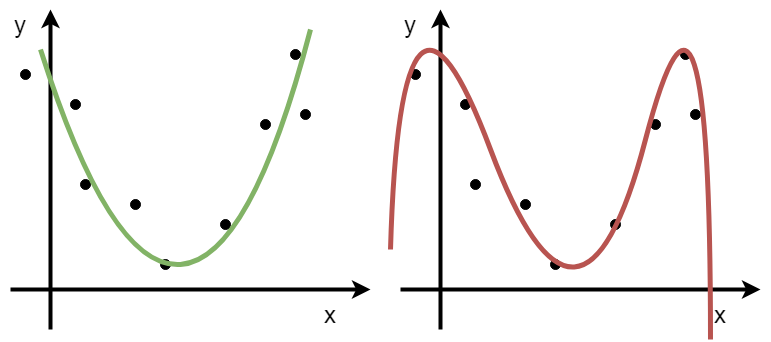
\includegraphics[width=10.0cm]{./8_appendix/img/regularization}
            \caption{Example of model behavior when overfitting occurs.}
            \label{2_overfitting}
        \end{center}
    \end{figure}
    例えば先程の例で以下の多項式を考えていた場合,$w_4$の値が大きくなったと考えられる.
    \begin{equation}
        h_{\bm{w}}(\bm{x}) = w_0 x^0 + w_1 x^1 + w_2 x^2 + w_3 x^3 + w_4 x^4 + w_5 x^5
    \end{equation}
    このように,特定のパラメータが大きくなりすぎることによって汎化性能が低下することを防ぐためにはモデルの正則化が重要である.
    
    モデルの正則化の発想は非常に単純で,損失関数にパラメータの値自体を組み込むことで,パラメータのスケールが必要以上に大きくなることを防ぐ.
    損失関数の中でも,特にこのような項を正則化項と呼ぶ.
    また,機械学習の枠組みではこのような正則化項の選び方を特に荷重減衰(weight decay)と呼ぶ.
    この正則化項を考慮した線形回帰の損失関数は以下のように表すことができる.
    \begin{equation}
        L(\bm{w}) = \frac{1}{2N}\sum_{i=1}^{N}\left(h_{\bm{w}}(\bm{x}^{(i)})-y^{(i)}\right)^2-\alpha \sum^M_{j=0}w_{j}^2
    \end{equation}
    ここで,$\alpha$は正則化の強さを決定するハイパーパラメータである.
    また,導出は省くが正規化項を考慮した正規方程式の解は以下のようになる.
    \begin{equation}
        \bm{w}=\left( \bm{\Phi}^T\bm{\Phi}+\alpha \bm{I} \right)^{-1}\bm{\Phi}^T\bm{y}
    \end{equation}
    また,上記の式では正則化項としてパラメータの二乗を用いているが,これは$|w_j|^q$として一般化できる.
    機械学習の枠組みではq=1のL1正則化,およびq=2のL2正則化がよく用いられる.
    統計学の分野においてはq=1のときを特にLassoと呼ぶ\cite{tibshirani1996regression}.
    このL1正則化(またはLasso)は,$\alpha$が十分に大きいときにいくつかのパラメータが0となる,疎な解が得られる.
    
\subsection{ロジスティック回帰}
    線形回帰は回帰を行うモデルであったのに対して,ロジスティック回帰は分類を行うモデルである.
    
    まず,分類問題の目標ベクトルについて考える.
    簡単のためにここでは二値分類を扱う.
    二値分類の場合,目標値は0または1になる.
    説明変数xのある値について0と1を分類する線形モデルは例えば,図\ref{2_classification}中における緑の線を描くようなモデルが考えられる.
    \begin{figure}[ht]
        \begin{center}
            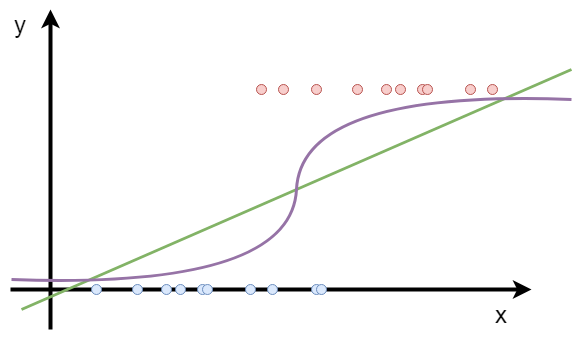
\includegraphics[width=10.0cm]{./8_appendix/img/classification}
            \caption{Schematic diagram of the classification model.}
            \label{2_classification}
        \end{center}
    \end{figure}
    しかし,このモデルはxを十分大きく(または十分小さく)した場合に1を超える(または0を下回る)ために,実用的とは言えない.
    以上から,出力が$0\leq h_w(x) \leq 1$となるようなモデル$h_w(x)$を考えるべきである.
    ここで以下の式で示されるsidmoid関数を導入する.
    \begin{equation}
        g(x)=\frac{1}{1+e^{-x}}
    \end{equation}
    この関数はロジスティック関数とも呼ばれ,図\ref{2_sigmoid}のような形状をしている.
    \begin{figure}[ht]
        \begin{center}
            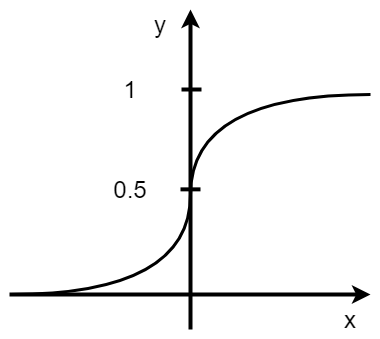
\includegraphics[width=7.0cm]{./8_appendix/img/sigmoid}
            \caption{Sigmoid function}
            \label{2_sigmoid}
        \end{center}
    \end{figure}
    
    線形回帰の出力にこのsigmoid関数を適用することにより,図\ref{2_classification}中における紫の線を描くようなモデルが得られる.
    ロジスティック回帰のモデルを線形モデルおよびsigmoid関数を利用して表現すると以下のような式になる.
    \begin{equation}
        h_{\bm{w}}(\bm{x}) = g\left(\bm{w}^T\bm{x}\right)=\frac{1}{1+e^{-\bm{w}^T\bm{x}}}
    \end{equation}
    つまり,閾値を0.5とすると,線形モデルの出力$\bm{w}^T\bm{x}$が正の値を取るときy=1と分類され,負の値を取るときy=0と分類される.
    以上から,入力空間はy=0となる境界により分割されることがわかる.
    このときの境界を決定境界(decision boundary),分割された領域を決定領域(decision region)と呼ぶ.
    簡単な例として,${w_,w_1,w_2}={-3,1,1}$とした際の分類境界を図\ref{2_classification_example}に示す.
    決定領域の中でも線形の決定面によって分離可能なデータ集合を特に線形分離可能(linearly separable)という.
    このとき,図\ref{2_classification_example}に示したように,入力データを加工することにより非線形境界も学習できることも注意したい.
    \begin{figure}[ht]
        \begin{center}
            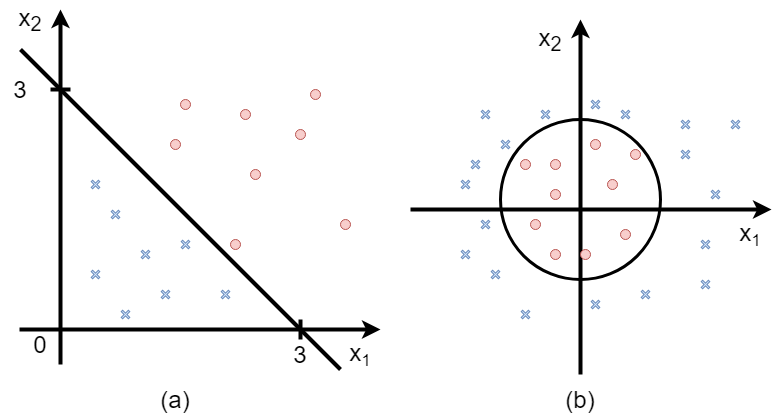
\includegraphics[width=12.0cm]{./8_appendix/img/classification_example}
            \caption{Classification boundary by logistic regression when the threshold is set to 0.5.\ (a)$x_1+x_2-3=0$\ (b)$x_1^2 + x_2^2-1=0$}
            \label{2_classification_example}
        \end{center}
    \end{figure}
    
    また,ロジスティック回帰におけるsigmoid関数のように,線形モデルに対して何かしらの変換を施す非線形関数のことを,機械学習分野では特に活性化関数(activation function)と呼ぶ.
    また,上記で見たように,活性化関数が非線形の場合にも,このモデルの決定境界は線形である.
    また,このようなsigmoid関数に限らない様々な非線形変換を線形モデルに施すことを想定した,ロジスティック回帰よりも一般化されたモデルのことを一般化線形モデル(generalized linear model\cite{mccullagh81nelder})と呼ぶ.

    ロジスティック回帰において決定境界を決定する$\bm{w}$は,線形回帰と同様に損失関数を最小化することによって導出できる.
    線形回帰は二乗誤差を利用して損失関数を定義したが,ロジスティック回帰において最小二乗誤差を利用するのは不適である.
    式\ref{linerregression_loss_equation}で表される損失関数において,線形モデルの場合,$h_{\bm{w}}(\bm{x})$は線形である.
    しかし,sigmoid関数を利用しているロジスティック回帰モデルの場合には,$h_{\bm{w}}(\bm{x})$は非線形となる.
    つまり,損失関数$L(\bm{w})$は非凸関数となり,局所解が増加し,大域解を求めるのが困難になる.
    \begin{figure}[ht]
        \begin{center}
            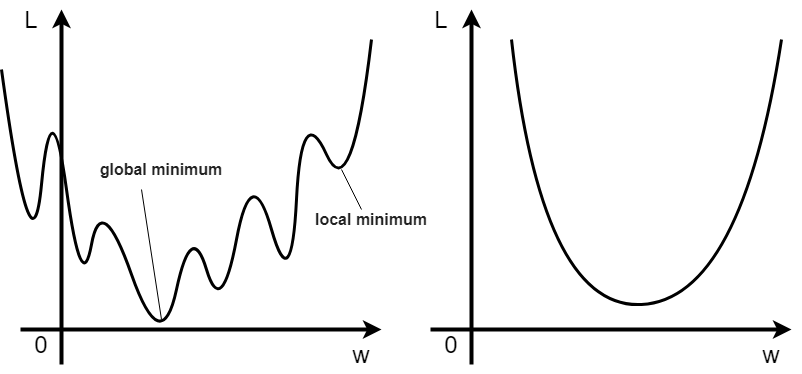
\includegraphics[width=12.0cm]{./8_appendix/img/global_minimum}
            \caption{Comparison of the solution space of the loss function by Mean Square Error when using linear and non-linear models.}
            \label{2_global_minimum}
        \end{center}
    \end{figure}
    
    そこで,分類タスクにおいては,以下のような損失関数を定義する.
    \begin{eqnarray}
        L\left(h_{\bm{w}}(\bm{x}), \bm{y}\right)=\left\{ \begin{array}{ll}
            -\log(h_{\bm{w}}(\bm{x})) & if\ y=1 \\
            -\log(1-h_{\bm{w}}(\bm{x})) & if\ y=0 \\
            \end{array} \right.
    \end{eqnarray}
    この損失関数は交差エントロピー誤差関数(cross-entropy error function)として広く知られている.
    この交差エントロピーを用いることによって誤差関数が収束することは,負の対数を図示すると直感的に理解できる.
    \begin{figure}[ht]
        \begin{center}
            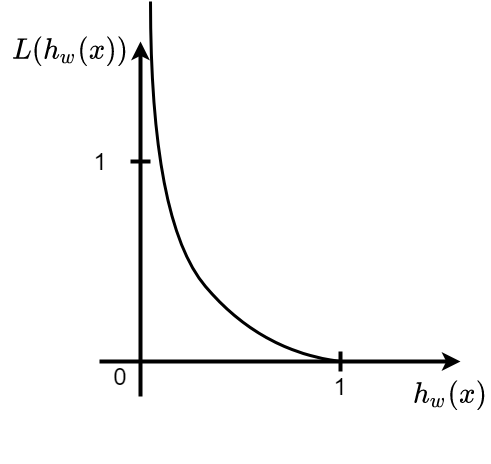
\includegraphics[width=7.0cm]{./8_appendix/img/log_negative}
            \caption{Loss function defined as a negative logarithm. (The domain is 0 <h (x) <1)}
        \end{center}
    \end{figure}
    
    この損失関数は計算機上で簡便に計算するために以下のようにも定義される.
    \begin{equation}
        L\left(h_{\bm{w}}(\bm{x}), \bm{y}\right)= -y \log(h_{\bm{w}}(\bm{x})) -(1-y)\log(1-h_{\bm{w}}(\bm{x}))
    \end{equation}
    つまり,各データの損失を考慮したときの一般化された損失関数は以下のようになる.
    \begin{equation}
        L(\boldsymbol{w}) = \frac{1}{N}\sum^N_{i=1}\left[-y^{(i)} \log(h_{\bm{w}}(\bm{x}^{(i)})) +(1-y^{(i)})\log(1-h_{\bm{w}}(\bm{x}^{(i)}))\right]
    \end{equation}
    
    さて,線形回帰と同様にロジスティック回帰についても微分値を求める.
    シグモイド関数の微分値は式\ref{sigmoid_eq}表すことができることに注意すると,損失関数の微分値は式\ref{logistic_loss_differential}で表すことができる.
    \begin{equation}
        \frac{\partial g(\boldsymbol{x})}{\partial \boldsymbol{x}} = g(x) (1-g(x))
        \label{sigmoid_eq}
    \end{equation}
    \begin{eqnarray}
        \frac{\partial L(\boldsymbol{w})}{\partial \boldsymbol{w}_j} 
        &=& \frac{1}{N}\sum^N_{i=1}\left[-y^{(i)} \frac{\partial \bm{z}}{\partial \boldsymbol{w}_j}\frac{\partial }{\partial \boldsymbol{z}}\log(\bm{z}) + (1-y^{(i)})\frac{\partial \bm{z}}{\partial \boldsymbol{w}_j}\frac{\partial }{\partial \boldsymbol{z}}\log(1-\bm{z})\right]\\
        &=& \frac{1}{N}\sum^N_{i=1} \left[-y^{(i)} h_{\bm{w}}(\bm{x}^{(i)})(1-h_{\bm{w}}(\bm{x}^{(i)}))\frac{\bm{x}^{(i)}}{h_{\bm{w}}(\bm{x}^{(i)})} \right.\\ 
        &&  \left.+(1-y^{(i)})(\bm{x}^{(i)})(1-h_{\bm{w}}(\bm{x}^{(i)}))\frac{h_{\bm{w}}(\bm{x}^{(i)}))}{(1-h_{\bm{w}}(\bm{x}^{(i)}))}\right] \\
        &=& \frac{1}{N}\sum^N_{i=1}\left(h_{\bm{w}}(\bm{x}^{(i)})-\bm{y}^{(i)}\right)\bm{x}^{(i)}_j
        \label{logistic_loss_differential}
    \end{eqnarray}
    この式は線形回帰の二乗和誤差と同じであることが分かる.
    
    さて,ここまでで二値分類の場合を考えてきたが,多クラス分類にロジスティック回帰を適用するのは至って簡単である.
    各クラスごとに,一対多の分類を行えば良い.
    これは本質的に今まで行っていた分類と何ら変わりがない.
    \begin{figure}[ht]
        \begin{center}
            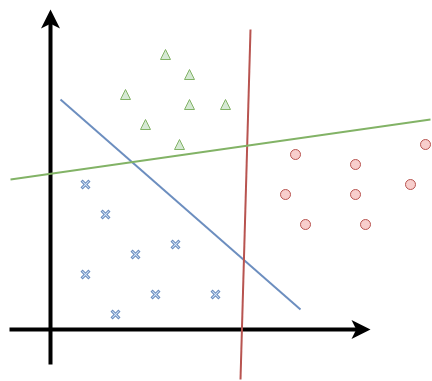
\includegraphics[width=8.0cm]{./8_appendix/img/one_vs_all}
            \caption{Overview of One-to-Many Classification.}
            \label{2_one_vs_all}
        \end{center}
    \end{figure}
    
    しかし,出力値の解釈には問題が生じる.
    ロジスティック回帰モデルは出力の範囲が$0\leq h_w(x) \leq 1$となるために,確率を出力するモデルとして考えることができる.
    つまり,ロジスティック回帰モデルの出力は$h_w(x)$は以下のような条件付き確率として表すことができる.
    \begin{equation}
        h_w(x)=P\left( y=k|x,w \right)
    \end{equation}
    ここで,kはクラスの値である.
    
    多クラス分類の際にそのまま一対多の分類を行った場合,各クラスの分類器が出力する値の合計は1を超える,または下回ることになる.
    そこで,各分類機の出力を正規化するために,ソフトマックス変換が用いられる.
    パラメータ$w$を持つ関数$h_w(x)$のクラス$k$に対する出力を$h^k_w(x)$とすると,ソフトマックス関数を用いて,各クラスに対する予測の条件付き確率は以下のように表すことができる.
    \begin{equation}
        P\left( y=k|x,w \right) = \rm{Softmax}(h^k_w(x)) = \frac{\exp{h^k_w(x)}}{\sum^K_{i=1}\exp{\left(h^i_w(x)\right)}}
    \end{equation}
    ここで,Kは合計のクラス数を表す.
    
    また,ロジスティック回帰の出力を確率値と捉えると,ロジスティック回帰は対数尤度を最大化するようにパラメータを学習していると捉えることができる.
    \begin{equation}
        \ln P=\sum_{n=1}^{N}\left\{y^{(n)} \ln \tilde{Y}\left(\mathbf{x}^{(n)} ; \mathbf{w}\right)+\left(1-y^{(n)}\right) \ln \left(1-\tilde{Y}\left(\mathbf{x}^{(n)} ; \mathbf{w}\right)\right)\right\}
    \end{equation}


